Après vous avoir introduit le contexte du projet, nous allons maintenant vous expliquer comment nous avons fait pour implémenter le crypto-système RSA.

\subsection{Implémentation sur 32 bits}
Comme nous l'avons vu dans la section précédente, pour implémenter le RSA, nous avons besoin des algorithmes suivant :
\begin{itemize}
	\item Exponentiation modulaire (déterminer $a$ tel que $a \equiv x^n \bmod n$);
	\item Inverse modulaire (étant donné $b$, trouver $a$ tel que $ab \equiv 1 \bmod n$).
\end{itemize}
Voici le pseudo code de ces deux algorithmes :

\begin{algorithm}[H]
\SetAlgoLined
\KwIn{base, exponent, modulus}
\KwOut{result}
$result \leftarrow 1$\;
$base \leftarrow base \mod modulus$\;
\While{$exponent > 0$}{
  \If{$exponent$ est impair}{
    $result \leftarrow (result \times base) \mod modulus$\;
  }
  $exponent \leftarrow exponent \div 2$\;
  $base \leftarrow (base \times base) \mod modulus$\;
}
\KwRet{$result$}\;
\caption{Exponentiation Modulaire}
\end{algorithm}

\begin{algorithm}[H]
\SetAlgoLined
\KwIn{a, m}
\KwOut{inverse modulaire}
$m0 \leftarrow m$\;
$y \leftarrow 0$\;
$x \leftarrow 1$\;
\If{$m = 1$}{
  \KwRet{$0$}\;
}
\While{$a > 1$}{
  $q \leftarrow a \div m$\;
  $t \leftarrow m$\;
  $m \leftarrow a \mod m$\;
  $a \leftarrow t$\;
  $t \leftarrow y$\;
  $y \leftarrow x - q \times y$\;
  $x \leftarrow t$\;
}
\If{$x < 0$}{
  $x \leftarrow x + m0$\;
}
\KwRet{$x$}\;
\caption{Inverse Modulaire}
\end{algorithm}

Nous pouvons voir que pour le premier algorithme, celui d'exponentiation rapide modulaire, nous utilisons un algorithme efficace contrairement à l'algorithme naïf qui consisterait a faire : $\underbrace{x \times x \times \ldots \times x}_{\text{n fois}}$. Afin de mettre en valeur la différence de complexité entre ces deux version, vous pouvez retrouver Figure \ref{fig:diff_complexite} la graphe représentant le nombre d'opération requis en fonction de l'exposant.
\begin{figure}[H]
    \centering
    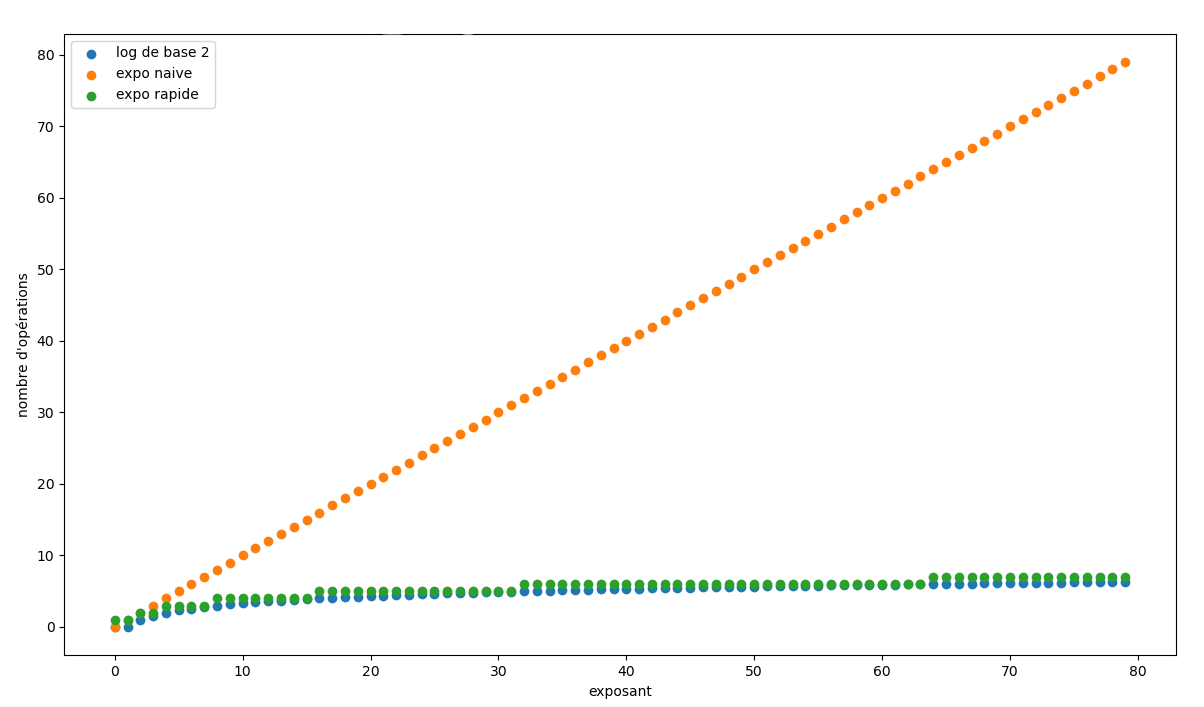
\includegraphics[width=\textwidth]{fig/diff_complexite.png}
    \caption{Comparaison des complexités des deux algorithmes d'exponentiation}
    \label{fig:diff_complexite}
\end{figure}
Il est aussi important de relever que la présence de l'algorithme d'exponentation rapide n'est pas un hasard, c'est grâce à lui que le système est faillible. En effet, si il rencontre un $1$ dans la représentation binaire du nombre il fait 2 calculs, sinon, il en fait 1 seul. Grâce à ça, il a une fuite de la clé qui s’opèrera sur la trace de consommation électrique.

Notre implémentation en C de ces deux algorithmes se trouve dans l'archive final du projet. Une fois ces primitives implémentées, il a été facile d'implémenter la génération de clé, le chiffrement et le déchiffrement, vous pouvez également retrouver ces implémentations en C dans l'archive final du projet.

\subsection{Objectif 2048 bits}
D'après les recommandation de l'ANSSI, un RSA implémenté avec les types de bases du C ($32$ bits), n'est pas du tout sécurisé
\subsection{Implémentation du big int}
\subsection{Conclusion}
